\subsection{Defining Key Terms}
The IoT landscape is often hard to understand, especially as names are defined loosely and  inconsistently. The same holds true for the cloud and terms around cluster technology. This section will explain the network topolgy, key terms and their concepts as the foundation for the following report.\\

\vspace{0.5mm}\\
\textbf\textit{Network Topology}\\
\cref{CNI} shows the network topolgy used in this report. The focus will be on the management and security of the device edge as well as its interaction with the IoT devices themselves. The upper layers like 
The infrastructure edge is mostly operated by network providers and are mainly used for networking purposes such as lower latency. As such, they are not directly related to IoT and relevant for this report.
On the contrary, the device edge is where the networking happens

\begin{figure}[h!]
    \centering
    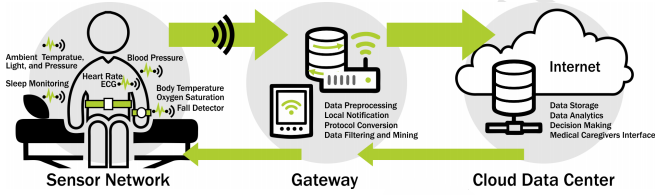
\includegraphics[scale=1.8]{figures/iotSetup.png}
    \caption{Network Topology inspired by \cite{iotGatewaySlavesGraph}.}
    \label{fig:netowrkTopology}
\includegraphics{}

\vspace{0.5mm}\\
\textbf{\textit{Constrained Device}}\\
Constraint devices are the elementary part of the IoT 
making up the "things" or devices\cite{contstraintDevicesTerminology}.
They can have three main purposes.
Either sensing or actuating (or both), where sensing is the 
passive action of measuring the environment (e.g. a motion detector) and actuating is the active action of influencing the environment (e.g. control of pressure in test tube). Or, finally, they can be smart objects enhancing the interaction between other smart objects and people.\\
They are usually defined by their limitation, mainly, small computing power (CPU, RAM, storage etc.) and limited power supply and operate in constrained network\footnote{See \cite{contstraintDevicesTerminology} page 5 for more information.}.\\
In summary, it is fair to assume that many constrained devices have very limited computing power, operate on battery in constrained networks using protocols like BLE and ZigBee. \\

\vspace{0.5mm}\\
\textbf{\textit{Smart devices}}\\
Smart devices are often not clearly defined in the academic literature, in this report I will use the definition given by \citeauthor{poslad2011smartDevices}\cite{poslad2011smartDevices}, to clearly divide them from constrained devices. They are traditional computing devices and "tend to be multi purpose ICT devices"\cite{poslad2011smartDevices}, examples are mobile phones (smart phones) or tablets. They connect to the rest of the infrastructure directly but are free to move between networks. They also often rely on battery power and, importantly, are mainly end user devices. This has important privacy implication when using their computing power for computations on the edge. \textbf{(I should pick this up somewhere in the report or go more in detail here).}\\

\vspace{0.5mm}\\
\textbf{\textit{IoT Gateway}}\\
IoT Gateways are the connection between smart devices and a network, this could be a local network or even the Internet. They facilitate inter-network and intra-network communications and because smart devices and especially constrained devices often communicate via wireless and non-Internet protocols, IoT gateways often translate protocols "between wireless sensor networks [...] traditional communication networks"\cite{zhu2010iotGatewayDefinition}.
In recent years IoT Gateways have become a major field of interest and new research. As these devices got more powerful, developers started using them for preprocessing and datagathering locally at the edge.
In conclusion, IoT gateways can take a wide variety of forms. They can be simple L3 routers or more powerful devices. Importantly, they are situated at the edge of a network and act as bridge between two autonomous systems.


\vspace{0.5mm}\\
\textbf\textit{Edge node}\\
Edge nodes are defined as nodes "that act as an end user portal for communication with other
nodes in cluster computing"\cite{Whatised17:edgeNodeDef}.
It operates on the edge, it must be able to run containers, has far inferior processing power compared to servers and can (only) run as a worker node (also known as a minion in kubernetes)\cite{NodesKub7:edgeNodeMinion}. Note that, this is in contrast to IBM which defines edge nodes as ingress traffic nodes in a cluster\cite{IBMCloudEdgeNodes0:online}.

Thus, in this report an edge node is a powerful IoT gateway situated at the edge of the network. But because of emerging technologies it will not be restricted by the type of software it can run (it can thus be a master node as well), but rather by its network topology and mobility. It is a node without reliable and fast connection to the rest of the network, does not need a static IP and is (somewhat) portable\footnote{Comparing edge nodes to cloud nodes is also common academic practice\cite{contstraintDevicesTerminology}  but not considered at this point.}.
Reoccurring themes are the restrictions compared to cloud clusters, which are smaller processing power,
no permament connection to the backbone network and greater portability.

\vspace{0.5mm}\\
\textbf\textit{Edge cluster}\\
The term edge cluster is closely related to cluster technologies like Kubernetes or Mesos.
Edge clusters are computers powerful enough to run a full control plane of the cluster technology.
However, there is no clear definition of what constitutes 
to an edge cluster in neither the academic literature nor the industry.
They are more powerful edge nodes, often packing additional hardware like GPUs or SSDs.
However, emerging technologies like tiny builds of a full Kubernetes cluster
like K3s from Rancher Labs\cite{k3sLight14:online} make this distinction 
between edge nodes and edge clusters
increasingly difficult
\footnote{Rancher provides a 40MB Kubernetes binary and claims that 500MB of RAM is sufficient 
it stable.}.\\
Because of their similarities, in this report the distinction between edge nodes and clusters will be solely
made up on the cluster topology separating them on an architectural level.

